\documentclass{standalone}
\standaloneconfig{border=2mm 2mm 2mm 2mm}

% PACKAGES: Maths
\usepackage{mathtools}
\usepackage{amsmath}
\usepackage{amssymb}
\usepackage{amsfonts}

% PACKAGES: tikzpicture
\usepackage{tikz}
\usepackage{scalerel}
\usepackage{pict2e}
\usepackage{tkz-euclide}
\usetikzlibrary{calc}
\usetikzlibrary{patterns,arrows.meta}
\usetikzlibrary{shadows}
\usetikzlibrary{external}

%PACKAGES: pgfplots
\usepackage{pgfplots}
\pgfplotsset{compat=newest}
\usepgfplotslibrary{statistics}
\usepgfplotslibrary{fillbetween}

%PACKAGES: colours
\usepackage{xcolor}
\usepackage{nicefrac}

\begin{document}

    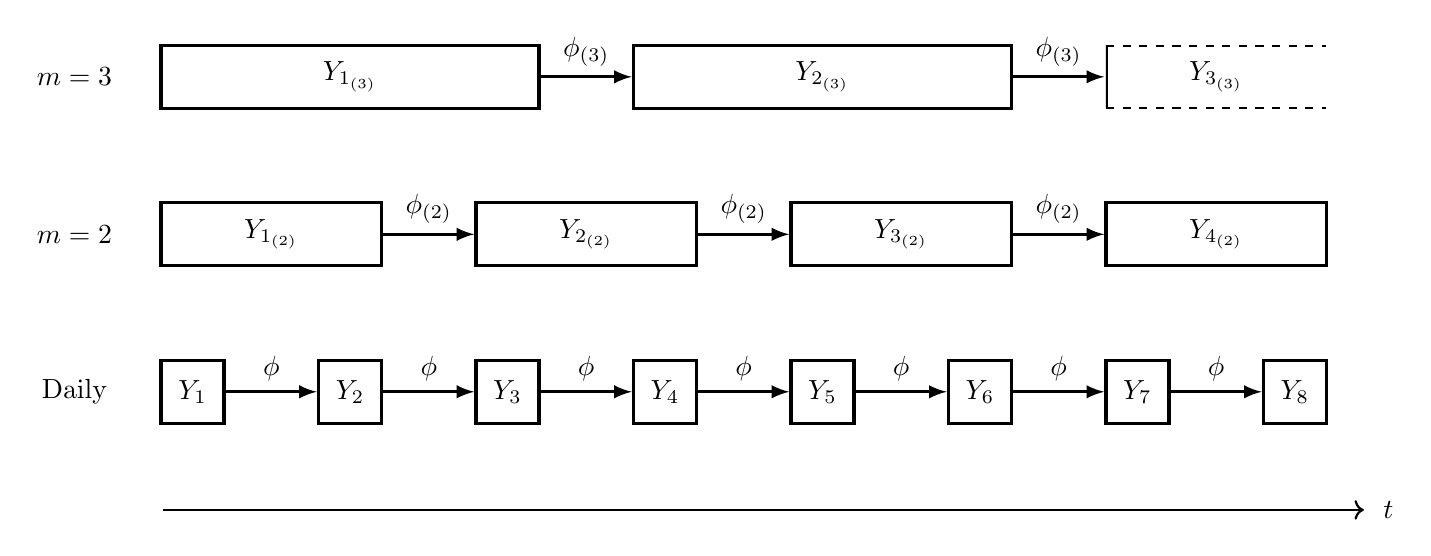
\begin{tikzpicture}[auto, scale = 0.5,
        time/.style={rectangle, inner sep=0pt, minimum size=8mm, align=center},
        manifest/.style={rectangle,draw,very thick,inner sep=0pt,minimum width=8mm,minimum height=8mm},
        paths/.style={->, very thick, -latex},
        openbox/.style={
            rectangle, very thick,
            minimum width=28mm, minimum height=8mm,
            path picture={
                \draw[dashed] (path picture bounding box.north west) -- (path picture bounding box.north east); % top line
                \draw[dashed] (path picture bounding box.south west) -- (path picture bounding box.south east); % bottom line
                \draw (path picture bounding box.north west) -- (path picture bounding box.south west); % left side
            }
        },
        double/.style={very thick, -latex}
    ]
    
        % Nodes
        \node[manifest] (y11) at (0,0) {$Y_{1}$};
        \node[manifest, right of = y11, xshift = 1cm] (y21) {$Y_{2}$};
        \node[manifest, right of = y21, xshift = 1cm] (y31) {$Y_{3}$};
        \node[manifest, right of = y31, xshift = 1cm] (y41) {$Y_{4}$};
        \node[manifest, right of = y41, xshift = 1cm] (y51) {$Y_{5}$};
        \node[manifest, right of = y51, xshift = 1cm] (y61) {$Y_{6}$}; 
        \node[manifest, right of = y61, xshift = 1cm] (y71) {$Y_{7}$};
        \node[manifest, right of = y71, xshift = 1cm] (y81) {$Y_{8}$}; 
                
        \node[manifest, above of = y11, yshift = 1cm, xshift = 1cm, minimum width=28mm] (y12) {$Y_{1_{(2)}}$};
        \node[manifest, above of = y31, yshift = 1cm, xshift = 1cm, minimum width = 28mm] (y22) {$Y_{2_{(2)}}$};
        \node[manifest, above of = y51, yshift = 1cm, xshift = 1cm, minimum width = 28mm] (y32) {$Y_{3_{(2)}}$};
        \node[manifest, above of = y71, yshift = 1cm, xshift = 1cm, minimum width = 28mm] (y42) {$Y_{4_{(2)}}$};
    
        \node[manifest, above of = y21, yshift = 3cm, minimum width = 48mm] (y13) {$Y_{1_{(3)}}$};
        \node[manifest, above of = y51, yshift = 3cm, minimum width = 48mm] (y23) {$Y_{2_{(3)}}$};
        \node[openbox, above of = y71, yshift = 3cm, xshift = 1cm] (y33) {$Y_{3_{(3)}}$}; % modified style for y33
    
        \node[left of = y11, xshift = -0.5cm] {Daily};
        \node[left of = y12, xshift = -1.5cm] {$m = 2$};
        \node[left of = y13, xshift = -2.5cm] {$m = 3$};
    
        % Paths: Autoregressive effects                
        \draw[paths] (y11) -- (y21) node[midway, above] {$\phi$};
        \draw[paths] (y21) -- (y31) node[midway, above] {$\phi$};
        \draw[paths] (y31) -- (y41) node[midway, above] {$\phi$};
        \draw[paths] (y41) -- (y51) node[midway, above] {$\phi$};
        \draw[paths] (y51) -- (y61) node[midway, above] {$\phi$};
        \draw[paths] (y61) -- (y71) node[midway, above] {$\phi$};
        \draw[paths] (y71) -- (y81) node[midway, above] {$\phi$};
    
        \draw[paths] (y12) -- (y22) node[midway, above] {$\phi_{(2)}$};
        \draw[paths] (y22) -- (y32) node[midway, above] {$\phi_{(2)}$};
        \draw[paths] (y32) -- (y42) node[midway, above] {$\phi_{(2)}$};
    
        \draw[paths] (y13) -- (y23) node[midway, above] {$\phi_{(3)}$};
        \draw[paths] (y23) -- (y33) node[midway, above] {$\phi_{(3)}$};
                
        % Time line                
        \node (timeline-start) [below of = y11, yshift = -.5cm, xshift = -0.5cm] {};
        \node (timeline-end) [below of = y81, yshift = -.5cm, xshift = 1cm] {};
         
        \draw[->, thick] (timeline-start) -- (timeline-end) node[midway, above] {};
        \node at (timeline-end) [right] {$t$};  % Add letter t to the right of the timeline
\end{tikzpicture}


\end{document}